% Exposé 0. Thesis (framework.md: "How to read this document" and "Exposé 0. Thesis"; site: 01-abstract.html)
\section{Thesis}\label{sec:thesis}

\begin{flushright}\small\itshape
The right generality turns a hard theorem into a remark,\\
and the remark into a design rule.\\[3pt]
{\upshape\footnotesize after Grothendieck}
\end{flushright}

Parameter-efficient fine-tuning (PEFT) has hundreds of methods, usually compared by parameter count and benchmark score. Those two numbers leave open what a method can reach, how it trains, and what happens to it when it is initialised differently, quantised, restarted or merged. Each of them becomes a precise mathematical question once a method is treated as a map, and many then have exact answers. This paper compares methods that way.

Fine-tuning moves a point. A pretrained checkpoint $\theta_0$ is a \emph{base point} in weight space $\Theta$, and a weight-space PEFT method is a \emph{relative object} over it, namely a pointed smooth map
\[
  \rho:(Q,q_0)\longrightarrow(\Theta,\theta_0),\qquad \rho(q_0)=\theta_0,
\]
from a small space $Q$ of trainable parameters into weight space. These maps form the pointed slice category $\Meth(\Theta,\theta_0)$ (\thmref{Definition}{I.2}). A morphism $h:M\to N$ is a pointed smooth map with $\rho_N\circ h=\rho_M$, read ``$N$ simulates $M$''. The frozen model is initial and full fine-tuning is terminal (\thmref{Observation}{I.4}), so every method pointed at $\theta_0$ sits in the interval between them. Following Grothendieck's relative point of view, the object of study is the morphism $\rho$ itself. Almost all the work is done by three invariants of the morphism, plus one further layer for architectures. Figure~\ref{fig:teaser} draws the picture.

The bicategory $\Para$ and the lens reading of backpropagation are due to \citet{fong2017backprop} and \citet{cruttwell2021categorical}. The closest earlier unified frame for PEFT is that of \citet{he2021unified}, who read adapters, prefix tuning and LoRA as modifications of specific hidden states. Ours works on the weight side, where adapters and prefixes return as extensions of the network (\thmref{Definition}{VI.1}).

\begin{figure}[tbp]
\centering
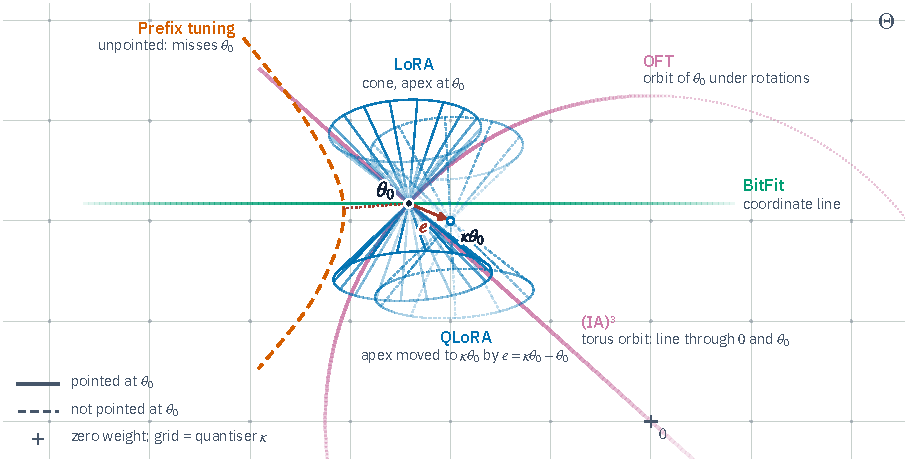
\includegraphics[width=\linewidth]{figures/teaser}
\caption{\textbf{Fine-tuning moves a point.} Weight space $\Theta$ is drawn as a chart around the pretrained point $\theta_0$; the grid is the lattice of a round-to-nearest quantiser $\kappa$ through the zero weight $0$ (marked $+$). Solid curves are image germs of methods pointed at $\theta_0$ (\thmref{Definition}{I.2}), drawn darkest near $\theta_0$ because only the germ there matters. LoRA \citep{hu2021lora} is the cone $\theta_0+\Mr$ with its apex at $\theta_0$ (\thmref{Theorem}{II.2}), shown as the rank-$\le1$ double cone $x^2=y^2+z^2$ of the symmetric $2\times2$ slice in perspective. OFT \citep{qiu2023controlling} is the orbit of $\theta_0$ under rotations, an arc of the circle about $0$ through $\theta_0$, the rest of which is dotted. (IA)$^3$ \citep{liu2022few} is a torus orbit, whose closure is the line through $0$ and $\theta_0$ (\thmref{Theorem}{II.5}). BitFit \citep{benzaken2021bitfit} moves along a coordinate line, parallel to the grid. The dashed curves are not pointed at $\theta_0$. Prefix tuning \citep{li2021prefix} extends the network and is unpointed (\thmref{Definition}{VI.1}); drawn in weight space it is a curve that misses $\theta_0$, at the distance marked by the dotted segment. QLoRA \citep{dettmers2023qlora} is LoRA pointed at the nearest grid node $\kappa\theta_0$, so its cone is LoRA's cone translated by the defect $e=\kappa\theta_0-\theta_0$ (red arrow), and $\theta_0$ is off its image unless $\rk e\le r$ (\thmref{Proposition}{V.2}).}
\label{fig:teaser}
\end{figure}

\subsubsection{Three invariants and one further layer}

The three invariants answer three practical questions: what a method can say, how it learns, and how it travels.

\paragraph{The image germ at $\theta_0$ governs expressivity}
This is what a method can say. Near $\theta_0$, the weights a method reaches form a linear space, a cone, a group orbit, a torus saturation, or a meet of these. Four data are read off this germ: the first-order image $S_1$, the expressive dimension $d(M)$, the min-cut bound on rank (the cut-rank), and the type of the base point, which is either a smooth point or an apex. Zero-initialised LoRA \citep{hu2021lora} starts at the apex of the cone $\theta_0+\Mr$, where first steps miss directions that the method reaches later; a PiSSA-style split \citep{meng2024pissa} starts at a smooth point. Exposé~\ref{sec:image} treats the germ in three parts: strata of initialisations (\ref{sec:strata}), invariants of group-type methods (\ref{sec:erlangen}), and cut and volume (\ref{sec:cut}).

\paragraph{The fibres, together with a metric, govern dynamics}
This is how a method learns. Many parameter values give the same weight, and the fibres of $\rho$ are gauge orbits; on LoRA's full-rank locus they are the orbits of $\GL_r$ acting by $g\cdot(B,A)=(Bg^{-1},gA)$. Combined with the optimizer's learning rates $\Lambda\succ0$, the parametrisation induces a cometric on weight space,
\[
  K=D\rho\,\Lambda\,D\rho\T ,
\]
so isomorphic methods can train differently. For LoRA with per-block rates, the compact half of the gauge acts by isometries and the non-compact half gives charges conserved under gradient flow. The optimizer's equivariance group decides what descends to the model (Exposé~\ref{sec:fibres}). The lens structure of backpropagation sorts tangent-side from cotangent-side methods (Exposé~\ref{sec:lens}). Through this lens, GaLore \citep{zhao2024galore} with no weight decay and no full-gradient clipping is one-sided LoRA with a moving frozen factor and carried-over optimizer state (\thmref{Proposition}{IV.2}); this identity is due to \citet{xtorrobahennigen2025duality}. This layer rests on work on factorised and linear networks: balancedness \citep{du2018algorithmic,arora2018optimization}, symmetries and conservation laws \citep{kunin2020neural,zhao2022symmetries}, and imbalance at initialisation \citep{xtarmoun2021understanding,xmin2021explicit}.

\paragraph{Base change moves $\theta_0$}
This is how a method travels. Initialisation by splitting, quantisation, restarts and merging all move the base point (Exposé~\ref{sec:base}). QLoRA \citep{dettmers2023qlora} is LoRA pointed at the quantised weights $\kappa\theta_0$, with defect $e=\kappa\theta_0-\theta_0$, and its image misses $\theta_0$ whenever $\rk e>r$, which is the generic case (\thmref{Proposition}{V.2}). Merge-and-restart with a fixed adapter shape reaches, in the limit, the orbit of the monoid generated by one cycle. For ReLoRA \citep{lialin2023relora} this means that $K$ cycles reach exactly the updates of rank at most $\min(Kr,m,n)$ (\thmref{Theorem}{V.3}).

\paragraph{Extensions and mergeability}
The fourth layer is the one place where a method changes the network $f$ itself; the network otherwise enters only through its realisation map and the backpropagation lens (\thmref{Remark}{I.3}). Adapters, prefixes and ReFT first extend $f$. Merging is then a lifting problem, certified by a local rewriting calculus of seven rules with side conditions, which gives sufficient conditions and box-local obstructions (Exposé~\ref{sec:merge}).

\subsubsection{Contributions}

Each result below is proved in Appendix~\ref{app:proofs}, and the scope stated here is the scope of the proof. Where a result, or a part of one, is due to others, the item says so. We re-derive such results in our language and add only their reading for fine-tuning.

\begin{enumerate}[label=\textbf{\arabic*.},leftmargin=1.9em]
\item \textbf{A relative frame for PEFT.} Weight-space methods are the objects of the pointed slice $\Meth(\Theta,\theta_0)=\Diff_*/(\Theta,\theta_0)$. Every such method lies in the interval [frozen, full FT], and ``$N$ simulates $M$'' becomes an explicit pointed map $h$ with $\rho_N\circ h=\rho_M$ (\thmref{Definition}{I.2}, \thmref{Observation}{I.4}). Isomorphism invariants finer than the image, such as $S_1$ and the singular locus, separate initialisations that the image cannot (\thmref{Observation}{I.6}, \thmref{Theorem}{II.2}). A categorical product produces a named method. Freezing either frame of LoRA gives two one-sided methods whose product is the sandwich $R\mapsto W_0+B_0RA_0$, which is LoRA-XS \citep{baazy2024lora} in the SVD frames of $W_0$ (\thmref{Proposition}{I.8}). Image-level meets, which are not products, organise others, such as HRA below. The bicategory $\Para$ is that of \citet{fong2017backprop} and \citet{cruttwell2021categorical}; the slice for PEFT and its invariants are new.

\item \textbf{No initialisation buys rank above $2r$} (\thmref{Theorem}{II.1}). For an additive method, moving the starting point while subtracting a frozen residual keeps the method pointed at $\theta_0$, and the union of all such re-pointed images is $\theta_0$ plus the difference set $C-C$ of its update shape. For $\mathrm{LoRA}_r$ that difference set is the matrices of rank at most $\min(2r,m,n)$. So no exact pointing of $\mathrm{LoRA}_r$, zero-init or split (PiSSA, OLoRA \citep{buyukakyuz2024olora}, CorDA \citep{yang2024corda}, LoRA-GA \citep{wang2024lorab}), makes an update of rank above $2r$ reachable in any adapted matrix, and split initialisations attain $2r$ when $2r\le\min(m,n)$. The statement is elementary; the $2r$ bound underlies the PiSSA-to-LoRA conversion of \citet{meng2024pissa}, implemented in Hugging Face (HF) PEFT.

\item \textbf{Three strata of initialisations, and two apexes} (\thmref{Theorem}{II.2}, \thmref{Theorem}{II.7}; Figure~\ref{fig:apex}). For LoRA of rank $r<\min(m,n)$ on one $m\times n$ weight there are three strata of exact full-rank pointings: $B_0=0$ with full-rank $A_0$ (vanilla LoRA on linear layers, EVA \citep{paischer2024parameter}); $A_0=0$ with full-rank $B_0$ (Init[B] \citep{hayou2024impact}, HF's default on embedding layers); and a rank-$r$ product $B_0A_0$ subtracted from the frozen weight (PiSSA, MiLoRA \citep{wang2024milora}, OLoRA, CorDA, LoRA-GA, Astra \citep{liu2026astra}). Two pointed LoRA methods in these strata are isomorphic over weight space exactly when they share $\operatorname{row}A_0$, $\operatorname{col}B_0$ or $B_0A_0$ respectively, so as a set the classes are $\Gr(r,n)\sqcup\Gr(r,m)\sqcup\MM_r$. Zero-factor pointings sit at the apex of the cone $W_0+\Mr$ and miss $r(n-r)$ or $r(m-r)$ first-order directions; split pointings sit at a smooth point, and neither image contains the other. The classification is set-level and in exact arithmetic. Rank-deficient pointings such as HF's \texttt{orthogonal} init, frozen-factor sub-objects (LoRA-FA \citep{zhang2023lora}, MiCA \citep{rudiger2026mica}) and quantised-base defects (QLoRA, LoftQ \citep{li2023loftq}) lie outside the three strata.

Let $W_0$ have full column rank and let $r$ be even with $2\le r\le n-2$. Then the image of $r$-reflection HRA \citep{yuan2024bridging} without Gram--Schmidt, HF PEFT's default (\texttt{apply\_GS=False}), is exactly $\{W_0R:R\in\SO(n),\ \rk(W_0R-W_0)\le r\}$. This is the image-level intersection of $\mathrm{LoRA}_r$ with the rotation orbit $W_0\cdot\SO(n)$, of dimension $rn-r(r+1)/2$, and HRA is not the categorical product of the two. At HF's default paired initialisation ($u_{2i-1}=u_{2i}$), $W_0$ is a singular vertex of the image and the first-order image has dimension $kn-k(k+1)/2$ with $k=r/2$, so that initialisation is an apex like zero-init LoRA. Both theorems are new.

\item \textbf{Exactly orthogonal methods keep the spectrum} (\thmref{Corollary}{II.6}, \thmref{Theorem}{V.3}). If every weight a method produces, including after merge-and-restart cycles, has the form $W_0R$ with $R$ exactly orthogonal on the input side, then in exact arithmetic the neuron Gram matrix $WW\T$ never changes. Every neuron norm, every angle between neurons (and with them the hyperspherical energy) and every singular value of $W_0$ stay fixed, however often the method is merged, and block OFT with a fixed partition also fixes each block Gram. This covers exact-Cayley OFT \citep{qiu2023controlling} and block OFT, strict GOFT \citep{ma2024parameter} without its optional scaler, HRA, and ETHER \citep{bini2024ether} as defined in its paper. It does not cover variants with a per-neuron or per-input scale (HF BOFT \citep{liu2023parameter}, HF OFT 0.14 to 0.15, GOFT's default code), output-side variants, or approximately orthogonal ones such as HF PEFT's default Cayley--Neumann OFT, qGOFT and ETHER+. With small generators each Cayley--Neumann merge is a contraction, so repeated merging can only shrink neuron norms and singular values; low-precision merges add rounding drift. The invariance itself is elementary, and preserving hyperspherical energy is the motivation of OFT \citep{qiu2023controlling}; new is the sorting of methods and implementations by whether they satisfy its hypothesis.

\item \textbf{Rank is a cut, dimension is a volume} (\thmref{Theorem}{II.10}, \thmref{Proposition}{II.12}; Figure~\ref{fig:rankvol}). The rank of a map computed by a tensor network is at most the smallest product of wire dimensions across any cut separating inputs from outputs (standard). The expressive dimension is at most the budget minus the dimension of the generic gauge orbit, with equality when the gauge is locally transitive on generic fibres. At equal budget, with $2r\le\min(m,n)$, $r^2\le\min(m,n)$ and $2r^2<m+n-1$, $\mathrm{LoHa}_{r,r}$ \citep{hyeonwoo2021fedpara} reaches at least $(m+n-1)-2r^2$ fewer dimensions than $\mathrm{LoRA}_{2r}$, about $m+n$ when $r^2\ll(m+n)/2$. It buys rank up to $r^2$ in exchange for $r\ge3$, and it is strictly dominated for $r\le2$. When $2r^2\ge m+n-1$, for example $r=64$ on $4096\times4096$ or LyCORIS-style $r=32$ on 320- to 640-wide layers, the dimension bound no longer separates the two, and wherever it is attained, as the numerical checks find, LoHa matches or exceeds $\mathrm{LoRA}_{2r}$ in dimension as well as in rank. GraLoRA \citep{jung2025gralora} ($k\times k$ blocks of rank $r/k$, HF default \texttt{hybrid\_r=0}) keeps LoRA's budget and dimension $r(m+n-r)$ and lifts the maximum rank to $\min(kr,m,n)$, but caps each block at rank $r/k$; for $k\ge2$ and $kr\le\min(m,n)$ neither image contains the other. The census is new.

\item \textbf{Kronecker sums cut the other way} (\thmref{Theorem}{II.11}; Figure~\ref{fig:cut}). Split the dimensions as $m=m_1m_2$ and $n=n_1n_2$. A $k$-term Kronecker sum $\sum_iC_i\otimes D_i$ is exactly a matrix of rank at most $k$ after the rearrangement of Van Loan and Pitsianis~\citeyearpar{loan1993approximation}, so unconstrained Kronecker methods are LoRA across a different cut of the same four-leg tensor. With equal square splits of a $d\times d$ weight, a generic rank-one update has the largest Kronecker rank, $d$, while the identity has Kronecker rank one. Hence zero-init $\mathrm{LoRA}_r$ and unconstrained $k$-term Kronecker sums, for $r,k<d$, have incomparable images. LoKr \citep{yeh2023navigating} updates $C\otimes BA$ with inner rank $r'\le\min(m_2,n_2)$ have rank at most $\min(m_1,n_1)\,r'$, attained, so LoKr's image lies inside that of zero-init $\mathrm{LoRA}_r$ exactly when $r\ge\min(m_1,n_1)\,r'$, and is incomparable with it otherwise when $\min(m_1,m_2)\min(n_1,n_2)>1$. The linear algebra is standard (the rearrangement and the operator-Schmidt decomposition); the PEFT reading is new.

\item \textbf{A conserved charge} (\thmref{Theorem}{III.5}, \thmref{Corollary}{III.6}, \thmref{Theorem}{III.9}; Figure~\ref{fig:noether}). With per-block rates, LoRA's charge
\[
  \Phi=B\T B/\eta_B-AA\T/\eta_A
\]
is conserved by every continuous-time update $\dot q=-\Lambda D\rho_q\T\gamma(t)$ with constant $\Lambda\succ0$, gradient or not, including minibatches, global-norm clipping and DoRA's \citep{liu2024dora} detached norm. The compact half of the gauge gives $\Lambda$-isometries that leave $K$ unchanged, so gauge-related initialisations give identical weight trajectories whenever the signal depends on $q$ only through $(t,\rho(q))$. With per-rank-channel rates, off-diagonal charges and isometries exist exactly between channels with equal products $\eta_{B,j}\eta_{A,j}$. Discrete steps make the charge drift, with relative drift of second order in the step size, and Adam and momentum are not covered. The law is a mild extension of known results: \citet[Prop.~5.1]{zhao2022symmetries} and \citet{marcotte2023abide}, after the balancedness principle of \citet{du2018algorithmic} and \citet{arora2018optimization} and the symmetry analysis of \citet{kunin2020neural}. New here is only the remark that $\gamma$ need not be a gradient. Under an isotropic charge the weight dynamics have a closed form, with a crossover scale below which zero-$B$ LoRA behaves like LoRA-FA; this closed form is due to \citet{xtarmoun2021understanding} and \citet{xmin2021explicit}, and the PEFT reading is ours.

\item \textbf{LoRA+ is $\alpha$ in disguise} (\thmref{Theorem}{III.10}, \thmref{Corollary}{III.11}; Figure~\ref{fig:orbit}). For zero-init LoRA under Adam with $\varepsilon=0$, no weight decay or clipping, one learning-rate schedule for both groups, and the same data order and dropout masks, LoRA+ \citep{hayou2024lora} with ratio $\lambda$ follows, in exact arithmetic, the same weight trajectory as LoRA with $\alpha$ multiplied by $\lambda$. Per-block $\varepsilon$ and decoupled weight decay keep the statement once they are rescaled too, and under SGD the factor is $\sqrt\lambda$. At a fixed rank, rsLoRA \citep{kalajdzievski2023rank} is LoRA with a rescaled $\alpha$ or $B$ learning rate; how $\alpha$ should scale with rank is a separate question. Both statements are instances of a hyperparameter torus: for a method whose update is $s$ times a multihomogeneous function of its parameter blocks, rescaling each block's initial scale and learning rate together with the overall scale $s$ (and, under Adam, the per-block $\varepsilon$, decoupled decay and clipping thresholds) leaves the weight trajectory exactly unchanged under Adam, given the same data order and dropout masks; under SGD the same holds with learning rates scaled by the square of the block factor. The LoRA/Adam case is due to \citet{schulman2025lora}; the general multihomogeneous torus and the SGD law are new.

\item \textbf{Adam sees a finite shadow of the gauge} (\thmref{Theorem}{III.3}, \thmref{Theorem}{III.12}, \thmref{Proposition}{III.4}; Figure~\ref{fig:gauge}). Gradient descent is natural exactly where cometrics agree, which for LoRA's linear gauge with block-scalar learning rates, at points where $A$ has full row rank and $r<n$, means exactly along $\Ort(r)$. On LoRA's full-rank locus with channel-uniform hyperparameters, the largest subgroup of $\GL_r$ under which the parameter update is equivariant is $\Ort(r)$ for SGD, with or without momentum, and the signed permutations $B_r$, of order $2^rr!$, for Adam and AdamW with any $\beta$'s, any $\varepsilon\ge0$ and decoupled decay. Positive diagonal rescalings become symmetries of Adam only jointly with per-rank-channel rescaling of the learning rates (and of $\varepsilon$ and learning-rate-coupled decay when these are nonzero), and only without global-norm clipping. Undamped scaled GD (Riemannian preconditioning) and LoRA-RITE \citep{yen2024lora} are equivariant under all of $\GL_r$; damping reduces scaled GD to $\Ort(r)$, and wrapping it in Adam reduces it to $B_r$. Combination rules must be gauge-natural as well. A rule for combining LoRA factors is a well-defined function of the adapters exactly when it is constant on the factorisation fibres, which task arithmetic on the products satisfies and post-hoc product-of-sums rules such as LoraHub \citep{huang2023lorahub} do not (\thmref{Proposition}{V.4}). The hierarchy is new; scaled GD is due to \citet{xtong2021accelerating} and, for LoRA, \citet{zhang2024riemannian}.

\item \textbf{GaLore is one-sided LoRA with a moving frame} (\thmref{Proposition}{IV.2}). If an adapter is linear in its trainable tensor ($W=W_k+\mathcal LC$ on the current base $W_k$, with $C_0=0$) and the optimizer depends only on the gradients it receives (SGD or momentum, Adam without weight decay, Adafactor without parameter scaling, no global-norm clipping, the same implementation on both sides), then training $C$ and merging gives exactly the same weights as running that optimizer on the compressed gradient $\mathcal L^*\nabla_WL$ and mapping back with $\mathcal L$. In particular, GaLore with weight decay $0$ is exactly one-sided LoRA whose frozen factor is GaLore's projector matrix, merged and re-initialised every period with the trainable factor's optimizer state carried over. Decoupled weight decay, parameter-scaled Adafactor, trust-ratio optimizers and full-gradient clipping break the identity, and Flora, which compresses only the momentum, is not covered. Known: \citet{xtorrobahennigen2025duality} for GaLore, and \citet{hao2024flora} for random projections.

\item \textbf{Base change has explicit defects and closures} (\thmref{Proposition}{V.2}, \thmref{Theorem}{V.3}; Figure~\ref{fig:rebase}). Quantising the frozen base moves the base point. At initialisation QLoRA misses the pretrained weight $W$ by the generically full-rank error $e=\kappa W-W$, and it can reach $W$ only if $\rk e\le r$. Splitting or error-fitting initialisations change this defect in an order-dependent way: split-then-quantise (QPiSSA) leaves $\kappa(W_{\mathrm{res}})-W_{\mathrm{res}}$, and one-step LoftQ leaves $e-s\,\mathrm{SVD}_r(e)$, which is $e$ minus its best rank-$r$ approximation only when the LoRA scale $s=\alpha/r$ is $1$, because HF's LoftQ initialisation ignores the scale. After $K$ merge-and-restart cycles with a fixed shape, the reachable set is $\theta_0+C^{+K}$ for an additive shape $C$, or $S^K\theta_0$ for a set $S$ of group elements containing the identity. Methods whose shape is a fixed subspace, subgroup or submonoid gain nothing, and ReLoRA reaches exactly $W_0+\{\rk\le\min(Kr,m,n)\}$. Exact-Cayley block OFT stays in $W_0\cdot\prod\SO(b)$, up to closure, unless its block hypergraph is connected, which BOFT's butterflies achieve only at full depth, and re-HRA reaches $(W_0+\MM_{\le Kr})\cap W_0\cdot\SO(n)$. New.

\item \textbf{The activation decides the merge} (\thmref{Theorem}{VI.3}, \thmref{Theorem}{VI.5}; Figure~\ref{fig:prefix}). A few exact rewrite rules give sufficient conditions for folding a scaling or affine PEFT edit into existing weights with no change in output. The feed-forward scale of (IA)$^3$ \citep{liu2022few} always folds into $W_{\mathrm{down}}$. It folds into $W_{\mathrm{up}}$ under SwiGLU or GeGLU for every scale and under ReLU for nonnegative ones, while under GELU only entries $0$ and $1$ fold. Position-selective edits (ReFT \citep{wu2024reft}, Activated LoRA \citep{greenewald2025activated}) and nonlinear adapters are not box-locally mergeable, and exactly merging a generic QLoRA or LoftQ update leaves the quantised format, with QA-LoRA \citep{xu2023qa} as the exception. For attention, a prefix \citep{li2021prefix} acts as an input-gated parallel adapter \citep{he2021unified} that rescales the content attention weights within its layer and never reorders them \citep{petrov2023prompting}, while LLaMA-Adapter's \citep{zhang2023llama} separate softmax with a zero-initialised gate leaves those weights unchanged. The rules are elementary, and the merge into $W_{\mathrm{down}}$ is noted by \citet{liu2022few}; SmoothQuant \citep{xxiao2023smoothquant} and AWQ \citep{xlin2024awq} already migrate scales through activations and meet the GELU obstruction. New is only the packaging as a merge calculus for PEFT, with explicit side conditions. The calculus gives sufficient conditions and box-local obstructions; deciding mergeability of a whole network lies outside its scope.

\item \textbf{An atlas} (Exposés~\ref{sec:examples}--\ref{sec:rosetta}, Appendix~\ref{app:catalogue}; Figures~\ref{fig:timeline} and~\ref{fig:graph}). Fourteen methods are worked through the three invariants. Seven coordinates, each read off a method's formula (kind, shape of the image germ, base point, gauge, covariance group, merge type and rebasing closure), classify \nMethods{} methods from \nPapers{} papers, \nHF{} of them in HF PEFT. The atlas records \nArrows{} simulation arrows between methods, each exhibited by an explicit map $h$ with $\rho_N\circ h=\rho_M$, and \nObstructions{} obstructions, each naming the test that rules an arrow out. The \nCore{} core methods form the periodic table and the category drawn in Figure~\ref{fig:graph}. A Rosetta stone translates between the PEFT and the categorical vocabulary.

\item \textbf{Predictions and limits} (Exposés~\ref{sec:predictions} and~\ref{sec:analogy}). The theory makes falsifiable predictions, each with its optimizer scope, and states plainly which of its words are analogies and which problems are open.
\end{enumerate}

Some further results are classical or standard and carry their credit in their headings: the complete invariants of the basic actions (\thmref{Theorem}{II.5}), the Kempf--Ness slice of the LoRA gauge (\thmref{Proposition}{III.7}; \citealp{xkempf1979length}) and the privileged basis fixed by an activation (\thmref{Lemma}{VI.2}).

\paragraph{Where the category theory earns its keep}
There are seven places.
\begin{enumerate}[label=\arabic*.]
\item The pointed slice gives the interval [frozen, full FT] for weight-space methods and makes ``simulation'' precise (Exposé~\ref{sec:slice}).
\item Isomorphism invariants finer than the image ($S_1$, the singular locus) classify initialisations (\thmref{Theorem}{II.2}).
\item A categorical product produces a named method (LoRA-XS, \thmref{Proposition}{I.8}), and image-level meets organise others (HRA, \thmref{Theorem}{II.7}).
\item Base change separates function-preserving reparametrisations, which act on the slice, from maps that move the base point (quantisers). The resulting pointing defects are elementary, but the slice makes their order dependence explicit (\thmref{Observation}{II.15}, \thmref{Proposition}{V.2}).
\item The lens 2-functor $\Para(\mathsf R)$ separates tangent-side from cotangent-side methods. The degree-one collapse shows that every cotangent method whose optimizer reads only its gradients (no weight decay, no parameter scaling, no full-gradient clipping) is, period by period, a forward linear method on a moving base (\thmref{Proposition}{IV.2}).
\item Naturality: gradient descent is natural exactly where cometrics agree (for LoRA's linear gauge with block-scalar rates, along $\Ort(r)$ where $A$ has full row rank and $r<n$), and combination rules must be gauge-natural (\thmref{Theorem}{III.3}, \thmref{Proposition}{V.4}).
\item Symmetric monoidal structure turns rank into a min-cut (\thmref{Theorem}{II.10}).
\end{enumerate}
The rest is real algebraic geometry, invariant theory, Lie generation and gradient-flow ODEs, and we say so where it happens. True but idle constructions are omitted: coends for the rank filtration, a saturation monad, sheaf language for locality, the Grothendieck construction $\int\Meth\to\mathbf{PNet}$, and coKleisli 2-cells for mixtures.

\subsubsection{How the results were checked}

Each of the \nPropositions{} numbered results was checked by adversarial model referees (Appendix~\ref{app:making-of}) against its proof, against the literature, and against the methods as published and as coded, including the source of HF PEFT at commit 85be3f3 of 30 September 2026. Of these, 14 stood as first written and 27 were repaired. A second round, with one mathematical and one faithfulness referee for each result, re-examined 26 of the repaired results and narrowed many of them. Its objections mostly concerned a side clause: a missing hypothesis, a remark that went past its proof, or a description of a method that matched only one implementation. For example, HF PEFT's LoftQ initialiser turned out to ignore the LoRA scale $\alpha/r$ (\thmref{Proposition}{V.2}). Only the narrowed forms are stated in this paper. Some results are new, such as the HRA apex; many are known and re-derived with credit, as the contributions above record.

\subsubsection{How to read this paper}

\paragraph{Plan}
Exposé~\ref{sec:slice} sets up the pointed slice and its invariants. Exposé~\ref{sec:image} studies the image germ: initialisations and their strata (\ref{sec:strata}), group-type methods (\ref{sec:erlangen}), and cut and volume (\ref{sec:cut}). Exposé~\ref{sec:fibres} treats fibres, metrics and training dynamics, Exposé~\ref{sec:lens} the backpropagation lens, Exposé~\ref{sec:base} base change, and Exposé~\ref{sec:merge} extensions and mergeability. Exposé~\ref{sec:examples} works through fourteen methods, Exposé~\ref{sec:atlas} gives the classification and Exposé~\ref{sec:rosetta} the Rosetta stone. Exposé~\ref{sec:predictions} lists falsifiable predictions, Exposé~\ref{sec:analogy} separates analogy from theorem and collects open problems, Exposé~\ref{sec:related} discusses related work and Exposé~\ref{sec:conclusion} concludes.

\paragraph{Labels}
Table~\ref{tab:labels} lists the labels. Every numbered item keeps the number it has on the companion site. Definitions, remarks and results share one counter within each exposé, so Definition I.2 is followed by Remark I.3 and Observation I.4.

\begin{table}[t]
\centering\small
\def\thesisbar#1{\textcolor{#1}{\rule[-0.35ex]{1.1pt}{2.2ex}}\enspace}
\caption{How to read the labels. The coloured rule is the one that marks the environment in the text.}
\label{tab:labels}
\begin{tabularx}{\linewidth}{>{\raggedright\arraybackslash}p{0.29\linewidth}X}
\toprule
\headrow \textbf{Label} & \textbf{What it means here}\\
\midrule
\thesisbar{tide}Theorem, Proposition, Lemma, Corollary & Proved in this paper, with the complete proof in Appendix~\ref{app:proofs}; the statement is set in italic. A heading that says \emph{known} and names authors marks a result due to them, which we re-derive in our language, adding only its reading for fine-tuning.\\
\thesisbar{tide!70}Observation & True and formally easy; kept because it organises.\\
\thesisbar{ochre}Definition & A definition.\\
\thesisbar{rulegray}Remark, Example & Commentary and instances, in upright type.\\
\thesisbar{wongpurple}Conjecture, [Conj] & A conjecture.\\
\thesisbar{wongvermillion!80}Prediction, [Pred] & A falsifiable prediction, stated with its optimizer scope.\\
\tikz[baseline=0pt]\draw[inkgray,line width=0.9pt,dash pattern=on 2.5pt off 2pt](0,-0.35ex)--(0,1.85ex);\enspace Analogy & Organising language with no theorem behind it. \emph{Noether}, \emph{Erlangen}, \emph{gauge} and \emph{moduli} are meant this way beyond what is proved (Exposé~\ref{sec:analogy}).\\
\textcolor{tide}{\sffamily\scriptsize\bfseries\textls[120]{WHAT THIS EXPLAINS}} & What a result says about methods as published and as implemented.\\
{[Num]} & Checked numerically in float64 (autograd Jacobian ranks, exact optimizer runs) by the ancillary script described in Appendix~\ref{app:repro}. The companion site's figures recompute their numbers in the browser.\\
{[Sketch]} & Only a proof sketch is given, in Appendix~\ref{app:proofs}; the claim is not counted as proved.\\
verified, repaired & Review status of a numbered result, recorded in the ancillary file \texttt{propositions.json}. Repaired results were corrected or narrowed, and only that form is stated.\\
\bottomrule
\end{tabularx}
\end{table}

\paragraph{Conventions}
These carry real weight in the arguments. Table~\ref{tab:notation} collects the notation.
\begin{itemize}
\item \emph{Linear box.} A linear box computes $y=Wx$ with $W\in\R^{m\times n}$, $m=d_{\mathrm{out}}$ and $n=d_{\mathrm{in}}$. Row $i$ of $W$ is output neuron $i$.
\item \emph{Two Gram matrices, two sides.} $K_{\mathrm{out}}(W)=WW\T$ is the neuron Gram matrix and $K_{\mathrm{in}}(W)=W\T W$ the input Gram matrix. A right multiplication $W\mapsto WR$ with $R\in\Ort(n)$ (the \emph{input side}) fixes $K_{\mathrm{out}}$. A left multiplication $W\mapsto PW$ fixes $K_{\mathrm{in}}$. Papers that store $W\T$ swap the words \emph{input} and \emph{output}; we translate every method into the convention above.
\item \emph{Ambient category.} Maps and dynamics live in $\Diff$. Images are taken in $\Set$. Every image we meet is semialgebraic, or definable in $\R_{\exp}$ when softmax is involved, so dimensions, smooth points and tangent cones are well defined.
\end{itemize}

\begin{table}[tbp]
\centering\small
\caption{Notation.}
\label{tab:notation}
\begin{tabularx}{\linewidth}{>{\raggedright\arraybackslash}p{0.19\linewidth}X}
\toprule
\headrow \textbf{Symbol} & \textbf{Meaning}\\
\midrule
$W$ & A linear box $y=Wx$, $W\in\R^{m\times n}$, with $m=d_{\mathrm{out}}$ and $n=d_{\mathrm{in}}$. Row $i$ is output neuron $i$.\\
$\Theta$ & Weight space, a real vector space of adapted and frozen boxes.\\
$\theta_0$, $W_0$ & The pretrained point; $W_0$ for one box.\\
$\rho$, $(Q,q_0)$ & The method, a pointed smooth map from trainable parameters $Q$ started at $q_0$, with $\rho(q_0)=\theta_0$.\\
$\Meth(\Theta,\theta_0)$ & The pointed slice $\Diff_*/(\Theta,\theta_0)$, whose objects are methods $M=(Q,q_0,\rho)$. A morphism $h:M\to N$ is a pointed smooth map with $\rho_N\circ h=\rho_M$, read ``$N$ simulates $M$''.\\
$\lvert M\rvert$ & The budget, $\dim Q$.\\
$d(M)$ & The expressive dimension $\dim\Im M=\max_q\rk d\rho_q$. The gap $\lvert M\rvert-d(M)$ is gauge waste.\\
$S_1$ & The first-order image $d\rho_{q_0}(T_{q_0}Q)$. The base point is regular if $\dim S_1=d(M)$, an apex if smaller.\\
$K$ & The induced cometric $D\rho\,\Lambda\,D\rho\T$, with $\Lambda\succ0$ the learning rates. Gradient flow is $\dot\theta=-K\nabla_\theta L$.\\
$K_{\mathrm{out}}$, $K_{\mathrm{in}}$ & The neuron Gram matrix $WW\T$ and the input Gram matrix $W\T W$.\\
$\Mr$, $\MM_r$ & Matrices of rank at most $r$; the smooth stratum of rank exactly $r$, of dimension $r(m+n-r)$. The singular locus of $\Mr$ is $\MM_{\le r-1}$.\\
$\mathrm{LoRA}_r$ & $\rho(B,A)=W_0+sBA$ with $B\in\R^{m\times r}$, $A\in\R^{r\times n}$ and $s=\alpha/r$.\\
$G$, $\GL_r$ & The weight gradient $\nabla_WL$; the LoRA gauge, $g\cdot(B,A)=(Bg^{-1},gA)$.\\
$T_m$, $T_m^+$ & The diagonal torus of invertible diagonal matrices; its identity component $\{\diag(d):d_i>0\}$.\\
$\mathrm{Diag}_m$ & The monoid of all diagonal matrices.\\
$\mathrm{Mon}_m$ & The monomial matrices, $T_m\rtimes S_m$.\\
$B_r$ & The signed permutations, $\{\pm1\}^r\rtimes S_r$, of order $2^rr!$.\\
$\CO(n)$ & The conformal orthogonal group $\R_{>0}\cdot\Ort(n)$; $\CO^+(2)\cong\mathbb C^\times$.\\
\bottomrule
\end{tabularx}
\end{table}

\paragraph{Proofs and appendices}
The main text contains no proofs. Complete proofs of all numbered results are in Appendix~\ref{app:proofs}, in the same order as the statements, one subsection per result. External theorems that the proofs use are quoted in Appendix~\ref{app:auxiliary}. Appendix~\ref{app:background} collects the background the paper assumes, on categories, monoidal categories and lenses, manifolds, germs and cones, and groups, symmetry and conservation; its entries keep the numbers A.1--D.34 they carry on the companion site, and readers new to category theory or Lie groups can start there. Appendix~\ref{app:catalogue} describes the catalogue and Appendix~\ref{app:repro} the numerical checks.

\paragraph{The companion site}
This paper is the long-form version of the interactive site at \url{[URL]}. The two share every number, so ``Theorem III.10'' names the same statement here, on the site and in the ancillary file \texttt{propositions.json}. The site states each result with its proof beneath it and has 20 interactive figures that recompute their numbers in the browser, among them an orbit explorer for LoRA+, a Gram lab for orthogonal methods, a gauge lab, Noether hyperbolas and a merge game. This paper gives the complete text, collects the proofs in Appendix~\ref{app:proofs}, and replaces the interactive figures by static ones. The catalogue, the arrows and obstructions, the numbered results with their review status, and the numerical checks accompany this paper as data files. When citing a result, please give its number; for a result marked known, please also cite the authors named in its heading, to whom the result itself is due.
